\renewcommand{\thealgorithm}{A.\arabic{algorithm}}
\chapter{Supplementary information}

\begin{table}[htbp]
    \centering
    \caption{The plane-wave cutoff convergence test for DFT calculations. The calculation of $\Delta E$ involves subtracting the previous energy, e.g. $\Delta E(450\,\mathrm{Ry}) = E(450\,\mathrm{Ry}) - E(400\,\mathrm{Ry})$. When the cutoff $\ge 800$ and the rel cutoff $\ge 60$, the error in total energy reduces to ca. 10\textsuperscript{-8} a.u. Only part of the results is shown for the sake of clarity.}
    \label{tab:cutoff-convergence-test}
    \begin{tabular}{cccc}
    \toprule
    \textbf{Cutoff (Ry)} & \textbf{Rel cutoff (Ry)} & \textbf{Total energy (a.u.)} & \textbf{\boldmath$\Delta E$ (a.u.)} \\
    \midrule
    400 & 60 & -2352.6355962810 & -- \\
    450 & 60 &  -2352.6262868887 & $9.31 \times 10^{-3}$ \\
    500 & 60 &  -2352.6262867349 & $1.54 \times 10^{-7}$ \\
    550 & 60 &  -2352.6254866602 & $8.00 \times 10^{-4}$ \\
    600 & 60 &  -2352.6243443853 & $1.14 \times 10^{-3}$ \\
    650 & 60 &  -2352.6242425582 & $1.02 \times 10^{-4}$ \\
    700 & 60 &  -2352.6224669798 & $1.78 \times 10^{-3}$ \\
    750 & 60 &  -2352.6209571227 & $1.51 \times 10^{-3}$ \\
    800 & 60 &  -2352.6212901605 & $-3.33 \times 10^{-4}$ \\
    850 & 60 &  -2352.6212901727 & $-1.22 \times 10^{-8}$ \\
    900 & 60 &  -2352.6212901873 & $-1.46 \times 10^{-8}$ \\
    950 & 60 &  -2352.6213082173 & $-1.80 \times 10^{-5}$ \\
    1000 & 60 &  -2352.6208957304 & $4.12 \times 10^{-4}$ \\
    \midrule
    10 & 800 & -2354.4562984779 & -- \\
    20 & 800 &  -2352.6775968461 & $1.78$ \\
    30 & 800 &  -2352.6281701514 & $4.94 \times 10^{-2}$ \\
    40 & 800 &  -2352.6213637375 & $6.81 \times 10^{-3}$ \\
    50 & 800 &  -2352.6212892865 & $7.45 \times 10^{-5}$ \\
    60 & 800 &  -2352.6212901605 & $-8.74 \times 10^{-7}$ \\
    70 & 800 &  -2352.6212901729 & $-1.24 \times 10^{-8}$ \\
    80 & 800 &  -2352.6212901739 & $-1.00 \times 10^{-9}$ \\
    90 & 800 &  -2352.6212901739 & $0.00$ \\
    100 & 800 &  -2352.6212901739 & $0.00$ \\
    \bottomrule
    \end{tabular}
\end{table}


\renewcommand{\algorithmicrequire}{\textbf{Input:}}
\renewcommand{\algorithmicensure}{\textbf{Output:}}
\begin{algorithm}[htbp]
    \caption{Density-aware sampling of configurations}
    \label{alg:density_aware_sampling}
    \begin{algorithmic}[1]
    \Require Feature matrix $\mathbf{X} \in \mathbb{R}^{N \times 2}$ of $N$ configurations, number of samples $n_\text{samples}$
    \State Determine number of clusters:
        \[
        k \gets \max\left(10, \min\left(\left\lfloor \frac{N}{50} \right\rfloor, \left\lfloor \frac{n_\text{samples}}{10} \right\rfloor\right)\right)
        \]
    \State Apply K-means clustering to $\mathbf{X}$ with $k$ clusters
    \State Initialize empty list for sampled cofiguration indices $S \gets [\ ]$
    \For{each cluster $C_i$, $i = 1$ to $k$}
        \State $n_i \gets \max\left(1, \left\lfloor \frac{|C_i|}{N} \cdot n_\text{samples} \right\rfloor \right)$
        \State Select $n_i$ random configurations from $C_i$ with fixed random seed
        \State Append selected indices to $S$
    \EndFor
    \State \Return $S$
    \Ensure List of selected configuration indices $S$
    \end{algorithmic}
\end{algorithm}



\begin{table}[htbp]
    \centering
    \caption{Composition of the full dataset used for training and testing. Well-tempered metadynamics settings used to run the simulations: \textsuperscript{1}GFN1-xTB for energies and forces, gaussian height = 2 kcal/mol, spawning frequency = 25 fs\textsuperscript{-1}, bias factor = 30 and  \textsuperscript{2}NNP for energies and forces, gaussian height = 2 kcal/mol, spawning frequency = 50 fs\textsuperscript{-1}, bias factor = 30.}
    \label{tab:full_dataset}
    \begin{tabular}{ccccc}
    \toprule
    \textbf{System} & \textbf{Temperature (K)} & \textbf{Simulation length (ps)} & \textbf{Train/Val} & \textbf{Test} \\
    \midrule
    MeDP\textsuperscript{1}  & 300 & 50 ps   & 2000 & 150 \\
    MeDP\textsuperscript{2}  & 300 & 100 ps & 2000 & 150 \\
    MeDP\textsuperscript{2}  & 320 & 500 ps  & 1000 & 300 \\
    MeDP\textsuperscript{2}  & 340 & 500 ps  & 1000 & 300 \\
    MeHDP\textsuperscript{1} & 300 & 50 ps  & 2000 & 150 \\
    MeHDP\textsuperscript{2} & 300 & 100 ps & 2000 & 150 \\
    MeHDP\textsuperscript{2} & 320 & 500 ps  & 1000 & 300 \\
    MeHDP\textsuperscript{2} & 340 & 500 ps  & 1000 & 300 \\
    \midrule
    \textbf{Total} & & & \textbf{12000} & \textbf{1800} \\
    \bottomrule
    \end{tabular}
\end{table}

\begin{figure}[htbp]
    \centering
    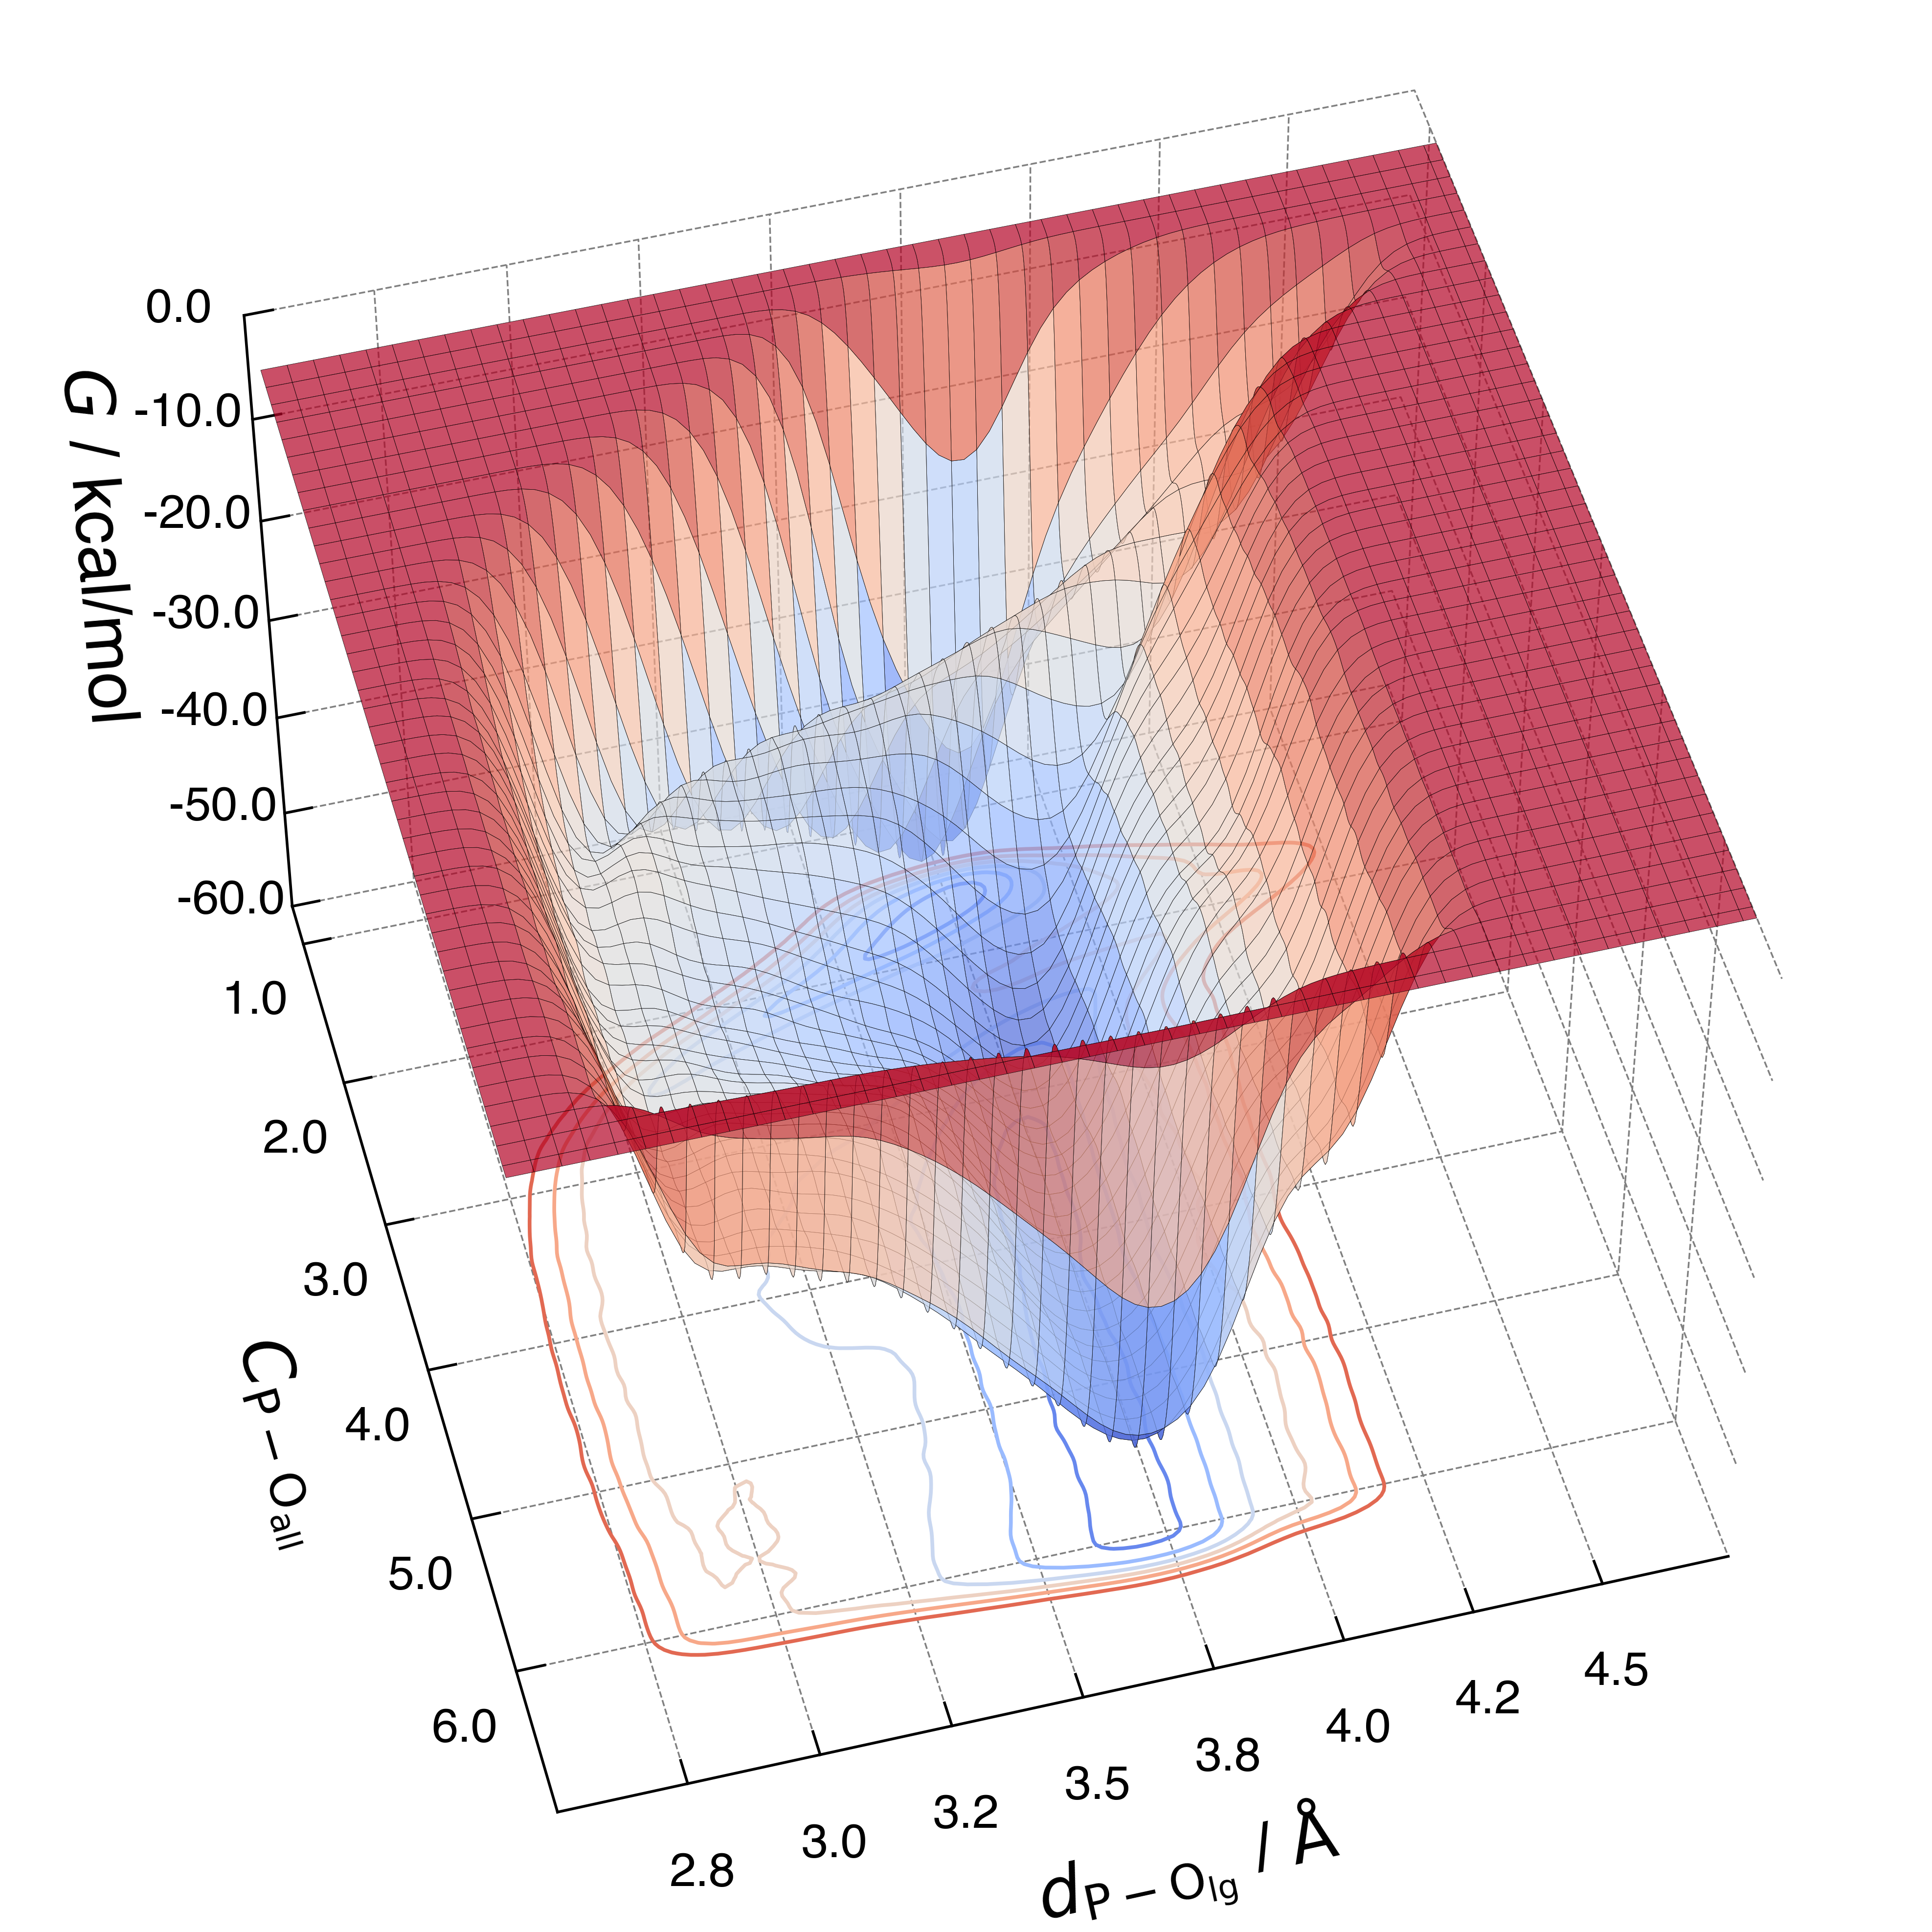
\includegraphics[width=0.65\textwidth]{Figures/Appendix/appendix_MeDP_300K_fes_3d.png}
    \caption{3D FES describing the hydrolysis of MeDP at 300 K.}
    \label{fig:fes_3d_medp_300k}
\end{figure}

\begin{figure}[htbp]
    \centering
    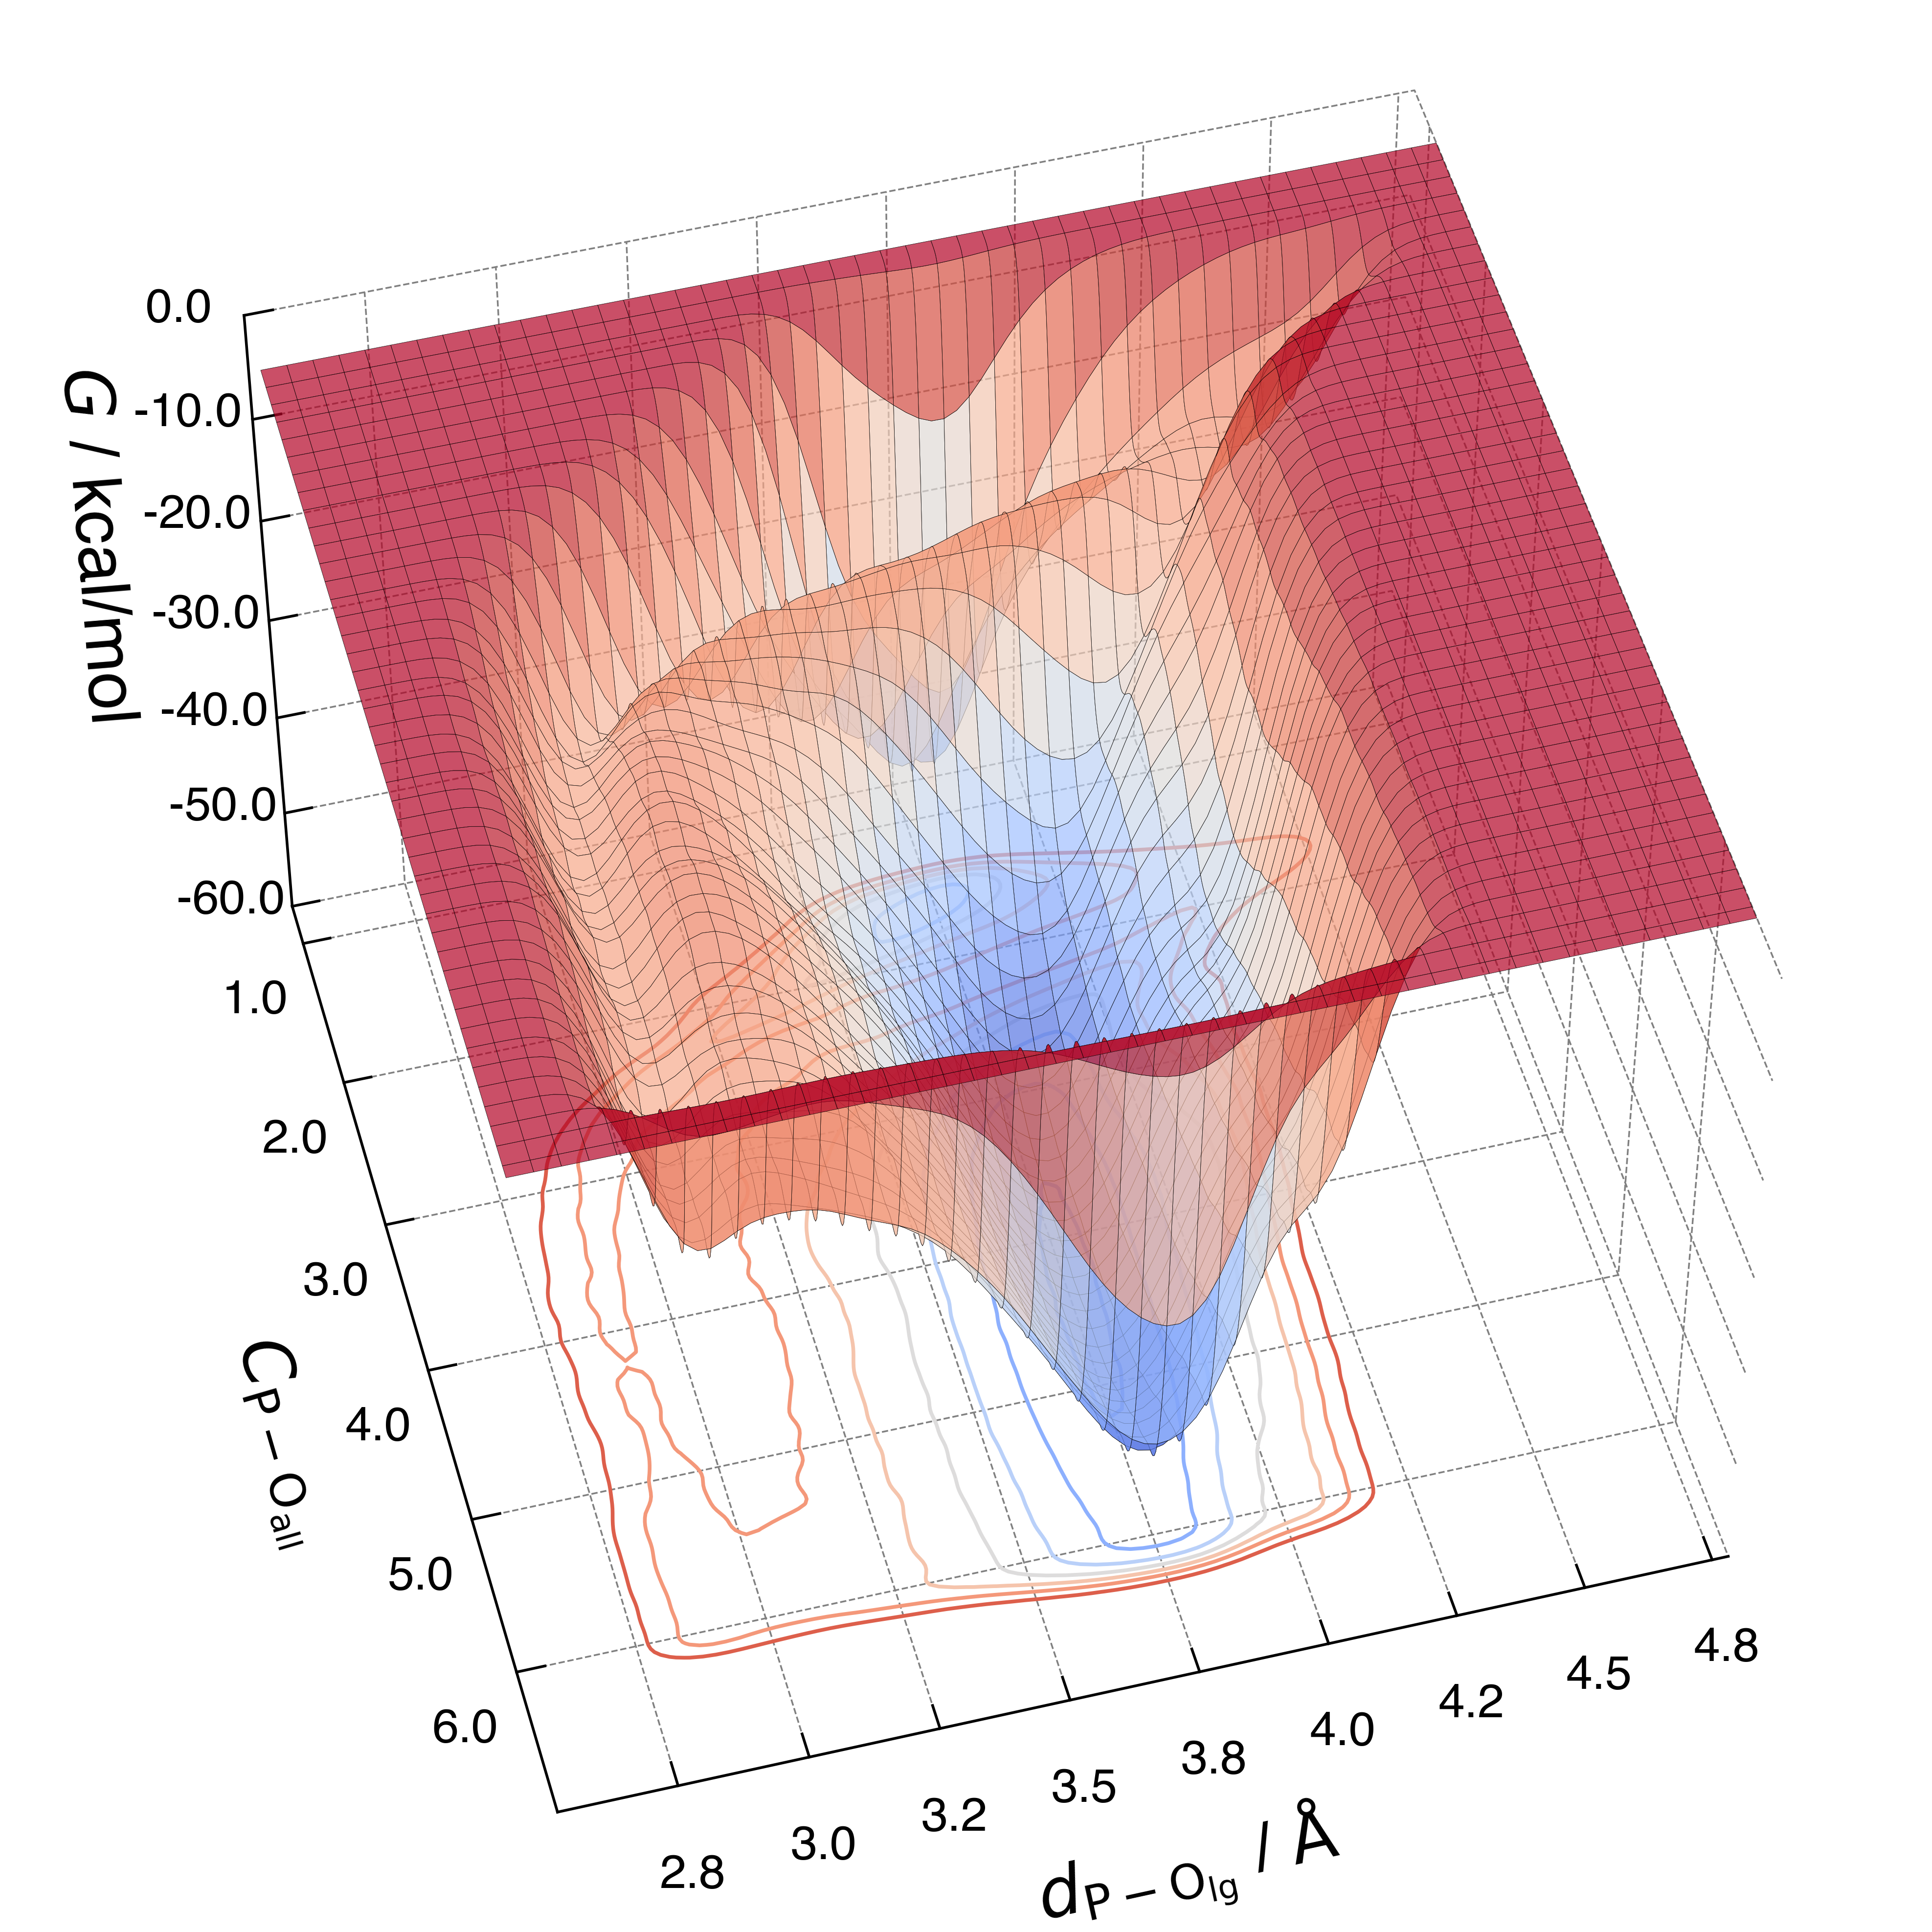
\includegraphics[width=0.65\textwidth]{Figures/Appendix/appendix_MeHDP_300K_fes_3d.png}
    \caption{3D FES describing the hydrolysis of MeHDP at 300 K.}
    \label{fig:fes_3d_mehdp_300k}
\end{figure}
